\newpage
\section{Algorithm Description}


There are two cases for the social influence problem, one in which the probabilities of the edges are known, and another in which they aren't and need to be learnt.

\subsection{Influence Maximization Problem}

In the known probabilities case, we can rely on the Influence Maximization algorithms.
In the last section there will be some graphs with all the different algorithms performance put in comparison.
We were not able to deeply analyse the problem because we are not able to run the CELFpp ( and even worse with the greedy ) when the number of nodes/edges increases too much (with a regular computer it was not possible to go further than 150).

\subsection{Online Influence Maximization Problem}

This scenario is the most similar to a real world problem.
We are given a network, in which we know the edges and the nodes, but we are not given the activation probabilities on those edges.
To solve this scenario, we can use an Explore/Exploit approach (bandit algorithms).
In this way, the algorithms aim at finding the best seed selection at each iteration for a given time horizon.
In the studied research, the scientific community uses a standard budget, we may call it K, that is the total budget to use.
They may run the online algorithm K times selecting only a single seed, K/2 times selecting 2 seed each time ..... 1 time selecting K seed at once.
We did not follow this approach, we went for a more streightforward way in which we indepedently selected K as a time horizon(number of times we can execute the algorithm), and k as the budget to use each time(number of seeds we can buy).

The framework of the problem is well explained in this picture:

\begin{figure}[H]
	\centering
	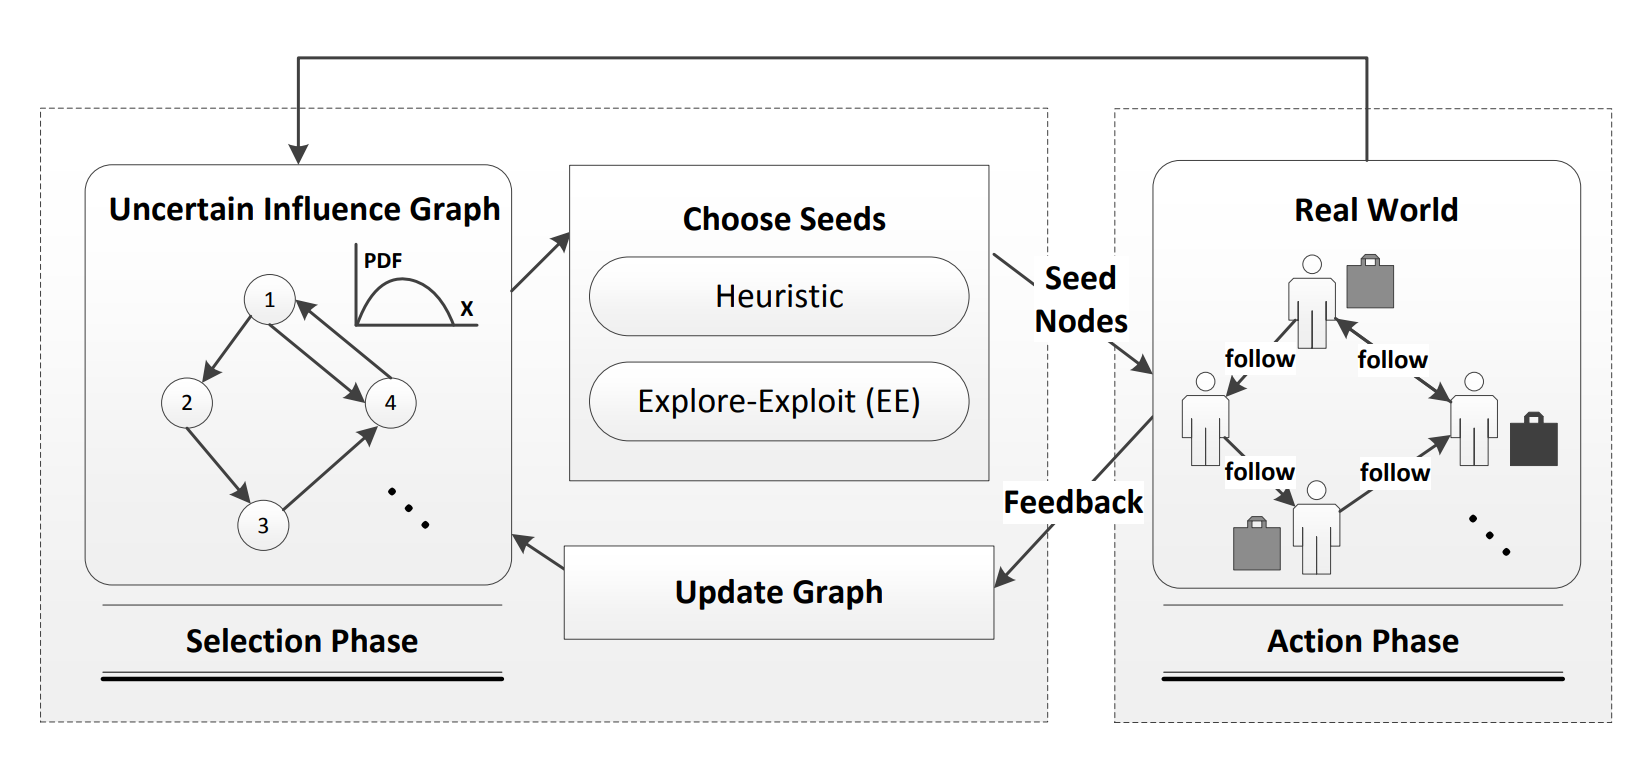
\includegraphics[scale=1]{img/IMG3}
\end{figure}

On the left there is the Uncertain Influence Graph, the network used by the algorithm to select the seed to buy.
From this graph then the seeds are selected, resolving the Influence Maximization Problem on the graph(see above), and are bought in the real world.
From the real world our environment can get the activation cascade information, which means it can see which edges have been activated by the selected nodes.
With this information, the algotrithm updates its Uncertain Influence Graph, and starts again until it reaches the end of the time horizon.
This is the pseuodocode of the Online Influence Maximization Algorithms, and should be straightforward to understand:

\begin{figure}[H]
	\centering
	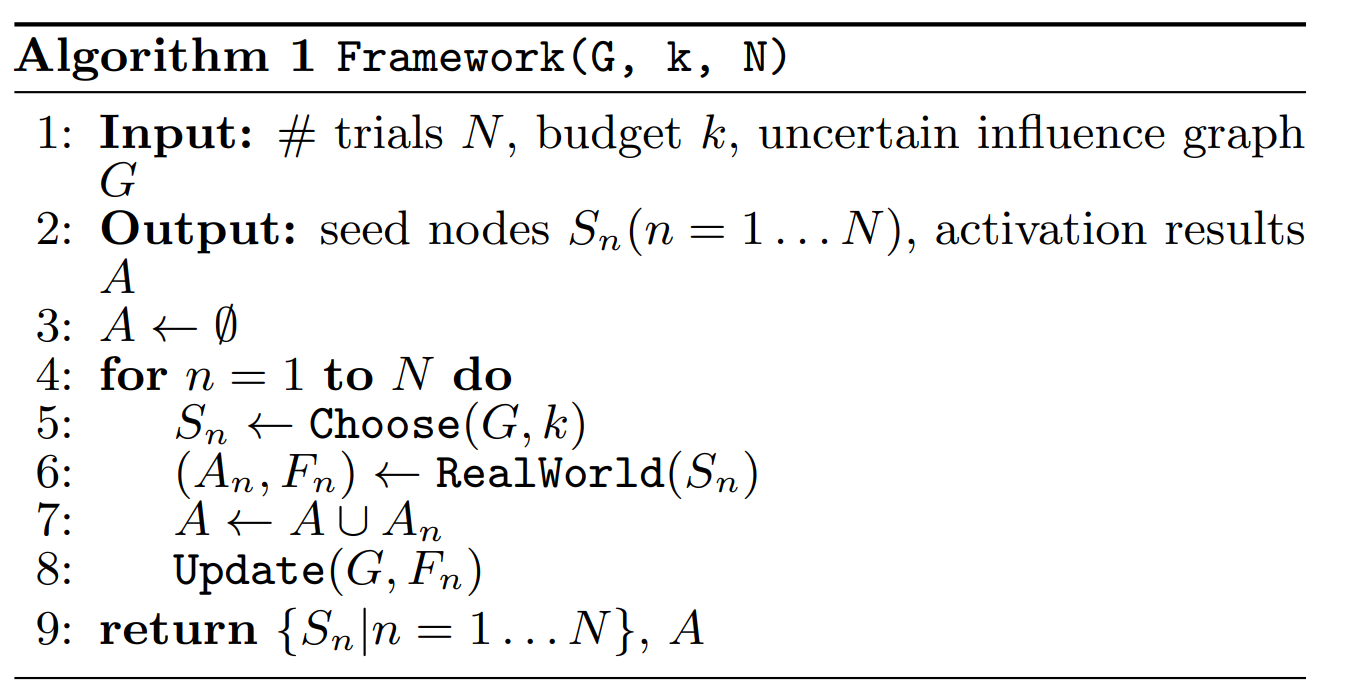
\includegraphics[scale=1]{img/IMG4}
\end{figure}


The problem is approached in two ways:

- In the first case we try to exploit the linear dependency of the edges with the theta parameters, in a linear regression manner, to learn the theta parameters that are common to all the edges.
In this case the feature vector of the edges is known, the algorithm LinearUCB every round learns a better approximation of the theta parameters value and can in this way do a better choice of the seed to select.
In this paper [3, Online Influence Maximization under Independent Cascade Model with Semi-Bandit Feedback, Zheng Wen, Branislav Kveton, Michal Valko, Sharan Vaswani] there is a more detailed explaination of how it works.

- In the second case, there is no exploit in the linear dependency of the theta parameters.
In this case the Combinatoria UCB and TS algorithms exploit in a standard way the network to select the seed set.
The difference between CUCB and CTS is in the way the edges probabilities on the Uncertain Influence Graph are calculated and updated.